
The Fourier Volume Reconstruction (FVR) method described in sections \ref{Sec:VolumeRegistrationSection} and \ref{Sec:AFVRApproach} was designed to be independent of RGB-D information input and thus sensors. As long as greyscale data with a depth component, RGB data with a depth component or depth data on their own are input, the FVR method should be able to compute accurate relative dense 3D reconstructions and optionally relative camera pose data. \\

Below, in section \ref{subsec:DSBR} both the advantages and limitations of 3D reconstruction via active depth sensors are discussed. It was discovered that the closer computed depth is to true depth (either via a stereo camera pair, active camera or monocular camera) the better the camera pose registration using the FVR method would be. Section \ref{subsec:SCBR} covers stereo input. Stereo pair computed depth has the potential to be the most accurate in terms of depth accuracy and resolution. Since the resolution only depends on the camera pair used, it can be high in contrast to active cameras. Budget active cameras such as the Microsoft Kinect and ASUS Xtion PRO LVIE camera, typically have a lower resolution than budget HD video cameras. \\

In section \ref{subsec:MVVRMethodology} the FVR is applied to monocular data. This technique is named Monocular View Volume Reconstruction (MVVR). The MVVR is discussed in terms of process and limitations in this section. Experiments in section \ref{Sec:MonocularExperimentsSection} show that the MVVR method is capable of camera translation tracking using noisy depth data generated using only monocular methods. However, its accuracy greatly depends on the quality of the 3D frames generated. \\

\subsubsection{Depth Sensor Based Reconstruction}
\label{subsec:DSBR}

Depth sensor input is advantageous for several reasons. It is faster to compute depth compared with both stereo and monocular methods, and in practice is more robustness and reliable. In most cases it is more accurate than monocular based methods. The major disadvantage in using such sensors has historically been one of accessibility. Thanks to budget active cameras such as the Microsoft Kinect and the Asus Xtion Pro Live camera being available to the general public at low cost, this is changing. However, there is still a mass of legacy video data which does not have actively generated depth data provided, moreover there is still a wealth of content still being produced by simple RGB cameras. \\

Another drawback of this sensor is that of accuracy. The accuracy of both the Kinect and Asus Xtion Pro Live sensors is limited to the resolution of the device. To alleviate this, some sub-pixel resolution generating algorithms may be used. These methods can be used in an attempt to generate greater resolution for given depth data. Methods may work on frames in a standalone fashion, although additional data such as consecutive frames and multi-camera techniques may also be used. Both the Microsoft Kinect and Asus Xtion Live Pro have maximum resolutions of $640 \times 480$. Methods of depth generation based on stereo data input are capable of generating dense depth information at resolutions only limited by the resolution of the cameras used. As of 2017, most cameras, even those found on mobile devices, can generate video data at resolutions of $1024 \times 1080$. \\

Another possible drawback in using RGB-D sensors is that certain materials reflect the infra-red light used by such active cameras to compute the depth information. These sensors are also known to produce noisy depth data around the corners and edges of objects captured within the frame. Since most computer vision algorithms make use of such salient features such as edges and corners within the image data, this can lead to inaccurate 3D reconstructions, especially in cases where 2D feature matching is used with RANSAC to produce 3D camera pose information. These sensors are also limited to indoor environments. If their infra-red sensor components are saturated with sunlight, little to no useful depth data may be generated. This is a major drawback as much of the world is made up of complex outdoor environments, therefore this is an unfortunate restriction given the usefulness of such cameras in indoor environments and lower light environments. \\

Another major disadvantage is that these sensors cannot produce depth data over distances. This is to do with the range of the active infra-red projection component of these sensors. Because the projection cannot reach far distances, the infra-red sensor cannot detect depth. This is in contrast to stereo and monocular methods which are capable of distant depth estimates.  

RGB-D camera sensors are still a popular choice for 3D reconstruction frameworks as the depth data produced by these methods is faster and more reliable than other sensors and techniques. For scenes and environments which can be accurately scanned by such depth sensors (such as environments with low sunlight, short ranges as in office environments and scenes with few objects which reflect infra-red light), RGB-D cameras are typically the preferred choice. The RGB-D data used to test the FVR method comes from an Asus Xtion Pro LIVE sensor. This sensor produces a colour and depth image input pair, which is processed in order to generate 3D volume frames which are the required input to the FVR method. \\

The color and depth image pair are referred to by $f(u,v)$ and $g(u,v)$ where $f(u,v)$ refers to the color image and $g(u,v)$ refers to the depth image. The colour image data contains a red, green and blue component each between the range $[0,255]$. Depth information is processed within the range $[0,10000]$. In terms of resolution, $u$ ranges $[0..639]$ and $v$ ranges $[0..479]$ giving a resolution of $640 \times 480$. Examples of images generated by the Asus Xtion Pro LIVE sensor are shown in figures \ref{fig:COLEXAMPLE} and \ref{fig:DEPTHEXAMPLE}. Given depth value for a given coordinate $u,v$, $Z_{u,v}$ is equal to the raw depth data value $g(u,v)$. Given coordinate $u,v$ and depth value $Z_{u,v}$ obtained via image $g$, $f(u,v)$ is projected into 3D space using equation \ref{eqn:PC_PROJECTION} to obtain the x-axis coordinate $X_{u,v}$ and y-axis coordinate $Y_{u,v}$. For each pixel value where depth information may be accurately recovered, the 3D point $[X_{u,v}, Y_{u,v}, Z_{u,v}]^T$ may be recovered. \\

From equation \ref{eqn:PC_PROJECTION}, the $X_{u,v}$ and $Y_{u,v}$ values are first translated relative to the center of the screen and then multiplied by the depth and attenuated by the focal length parameter. This is a typical projection function. In the equation, $c_x$ and $c_y$ represent the point where the optical axis intersects the projection plane (which occurs right at the center of the image, $c_x = 319.5$, $c_y = 239.5$. Parameters $f_x$ and $f_y$ represent the focal length which is defined as $f_x$, $f_y = 525.0$. \\


\begin{equation} \label{eqn:PC_PROJECTION}
\begin{split}
X_{u,v} & = \frac{(u - c_x)Z_{u,v}}{f_x} \\
Y_{u,v} & = \frac{(v - c_y)Z_{u,v}}{f_y} \\
\end{split}
\end{equation}

The FVR method requires that the point cloud generated by 3D points $[X_{u,v}, Y_{u,v}, Z_{u,v}]^T$ and colour data $f(u,v)$ be quantized for integration within a 3D volume. The volumes sizes used for testing were of sizes $128^3$, $256^3$ and $384^3$. Primarily, sizes $256^3$ and $384^3$ were used. It is common to use sizes which are an exponent of 2 for various computational reasons. However, $512^3$ was too large for the GPU used for testing (an NVIDIA GeForce 840 M GPU) so the maximum size $384^3$ was used for testing. The 3D point clouds were scaled to fit the volume, then their coordinates were rounded and integrated into the volume prior to registration. Examples of a colour and depth image pair as well as the corresponding projection into different volume sizes ($128^3$ and $256^3$) are shown in figure \ref{fig:PROJECTED_FRAME}.  \\

Once the data has been projected into a volume, it may be used as input to the technique described in section \ref{Sec:AFVRApproach}. The algorithm may then compute the registration matrix required to merge two frames, the matrix is accumulated and used to integrate each frame in succession. Upon registration and integration of each frame, the final output 3D reconstruction may be obtained. \\

\begin{figure}[!htb] 
        \centering
        \begin{subfigure}[b]{1.8in}
                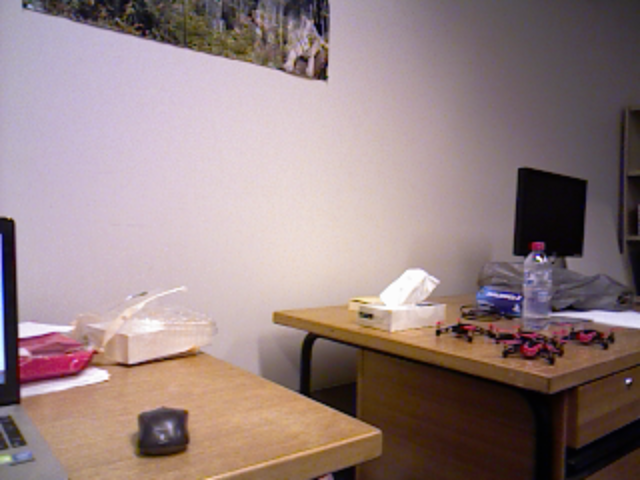
\includegraphics[width=1.7in]{images/ch2/colorF11}
                \caption{Color Image}
                \label{fig:COLEXAMPLE}
        \end{subfigure}%
        \begin{subfigure}[b]{1.8in}
                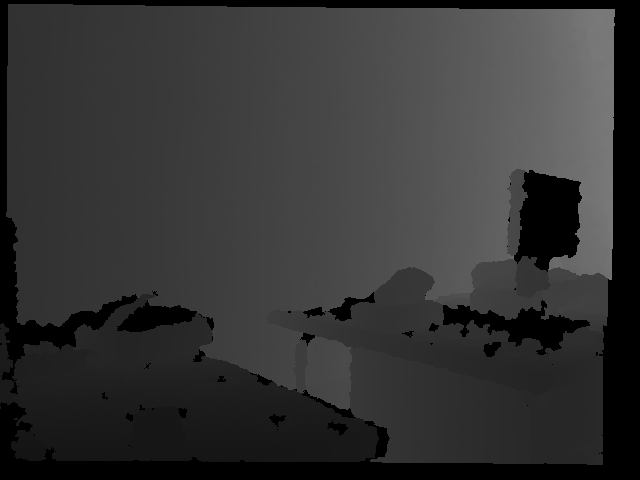
\includegraphics[width=1.7in]{images/ch2/depthF11}
                \caption{Depth Image}
                \label{fig:DEPTHEXAMPLE}
        \end{subfigure}
        
         \begin{subfigure}[b]{1.8in}
                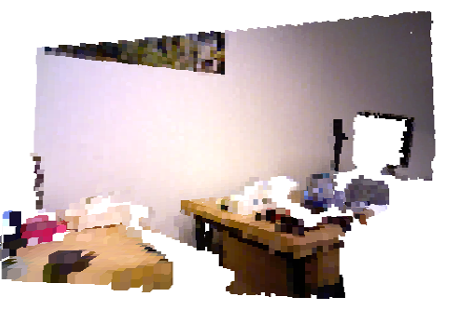
\includegraphics[width=1.8in]{images/ch2/volumeF11128}
                \caption{Projected Volume $128^3$}
                \label{fig:VOLUMEEXAMPLE128}
        \end{subfigure}%
         \begin{subfigure}[b]{1.8in}
                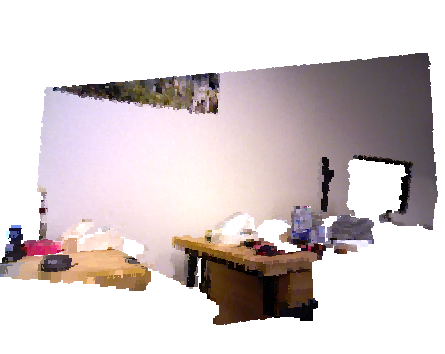
\includegraphics[width=1.8in]{images/ch2/volumeF11256}
                \caption{Projected Volume $256^3$}
                \label{fig:VOLUMEEXAMPLE384}
        \end{subfigure}%
       \caption{A Projected Frame.}
       \label{fig:PROJECTED_FRAME}
\end{figure}

\subsubsection{Stereo Camera Based Reconstruction}
\label{subsec:SCBR}
As mentioned, the FVR method may take dense depth data from any type of input sensor, as long as dense 3D point clouds can be generated per frame or near per frame rates 3D reconstructions may be computed. Stereo methods are capable of producing depth data at much higher resolitions and accuracies but are not as fast or as reliably compared to active sensors such as RGB-D cameras. However, they can produce depth maps under many environmental conditions where active cameras cannot. Outdoor scenes with a lot of sunlight may be captured with a stereo pair and used to compute dense depth data per frame. This data can then be integrated into the FVR algorithm. Additionally stereo sensors are capable of generating depth data over larger ranges as compared to active camera approaches. In this way, they can be used to scan objects in far off distances or produce depth data from overhead aerial data. \\

A major disadvantage is that in practical stereo algorithms, depth maps can be noisy. Computing 3D reconstructions from depth data which have been produced via stereo methods is also a challenging research project in itself. Still the noise is much lower in comparison to monocular methods of depth estimation. In generating depth data using a stereo set-up, the stereo camera pair must first be calibrated. The camera pair may be calibrated using software techniques to compute intrinsic camera parameters. Alternatively, the stereo data may be computed without first calibrating the stereo pair, resulting in less accurate depth data. Section \ref{StereoMethodsSection} described some of the available techniques in generating stereo data. \\

\subsubsection{Monocular View Volume Reconstruction}
\label{subsec:MVVRMethodology}

Generating dense depth information from monocular view is challenging. There are methods however, which take advantage of the properties of the Fundamental and Essential matrices to pre-calibrate consecutive frames. This allows stereo methods (see section \ref{StereoMethodsSection}) to be used to compute dense depth data per frame. These stereo methods are typically split into three categories: global, semi-global and local. Global methods are the most complex, and typically make use of some optimization method which optimizes the depth map's smoothness, disparity and contouring of edges jointly. Semi-global methods also optimize the depth map with respect to these requirements, however they are restricted to optimizing scan lines. This makes them much faster than the global optimization methods, whilst still providing better results than the local methods. Local methods are fast and ideal for real time applications, they make use of block matching to compute the disparity per pixel. \\

These methods all require frame by frame rectification. To do this, the fundamental matrix must be estimated accurately. The computation of the Fundamental matrix requires the use of feature matching and RANSAC which often are unable to accurately compute the Fundamental matrix. To generate dense depth data per frame, the use of optical flow based on 2D block matching was explored. By using 2D block matching, dense depth approximations were able to be computed whilst circumventing the use of the fundamental matrix and frame rectification. The depth maps computed are very noisy and inaccurate. The use of 2D spatial filtering as well as temporal filtering reduces such noise. \\

The spatial filtering technique used is basic Gaussian convolution. Temporal filtering was performed on a per pixel basis, where the output depth map is computed based on the previous depth map and the most recent depth map. Each depth map value is set to a value of $\delta \times prior-depth + (1-\delta) \times current-depth$. The best value for $\delta$ was judged based on qualitative analysis of experiment data sets. This method, although simpler and less accurate than other stereo methods, was used to test the FVR methods robustness to noisy and inaccurate 3D frame input. \\


For best performance, RGB-D information from alternative sources may be used in the FVR 3D reconstruction algorithm such as depth computed via active camera (Kinect, Asus Xtion LIVE PRO sensors) or disparity computed via stereo device. An alternative method is proposed here named Monocular View Volume Registration ($MVVR$). This algorithm takes consecutive RGB frames as input from a monocular camera sensor and computes depth data from them using the simple block matching method. The depth data is not aligned and because of camera speeds projection may not be consistent across frames. The depth maps are computed under the assumption of temporal camera translation. By performing block matching on frames taken from different camera locations, depth map be computed but only if the camera displacement is large enough. Therefore a $skip$ variable is used in order to block match frames with a distance from each other. \\

Using the computed depth maps, the algorithm projects consecutively computed depth maps into frames, which are then voxelized. Once the two frames are voxelized, the FVR technique proposed in sections \ref{FVRSectionA} and \ref{Sec:VolumeRegistrationSection}. A registration matrix may then be used to update camera parameters and to register and integrate the 3D frames. 

The algorithm is detailed in listings \ref{algorithm:MVVRAlgorithm}. A queue is used named $frameQueue$ to keep track of input RGB frames in order to generate depth data using frames which have a predefined temporal separation. A stack, $depthMapStack$ is used to keep track of the next two consecutive depth maps to register. $GlobalReconstruction$ is an automatic dynamically resizeable occupancy grid. \\

The matrix $M$ is used to keep track of the accumulation of transforms used to register and integrate each depth map into the global reconstruction output. Both $Camera_{location}$ and $Camera_{pose}$ keep track of the camera's location and pose information on a per frame basis. The list, $Cameras$ keeps track of the list of camera location and pose information for each frame.\\

\begin{figure}
\begin{lstlisting}[language=c++,caption=Monocular View Volume Reconstruction,label=algorithm:MVVRAlgorithm,mathescape,basicstyle=\ttfamily]
$frameQueue$ = newQueue();
$depthMapStack$ = newStack();
$GlobalReconstruction$.clear();
$M$ = IdentityMatrix();
$Camera_{location}$ = $[0, 0, 0]^T$;
$Camera_{pose}$ = $[[1, 0, 0]^T,[0, 1, 0]^T,[0, 0, 1]^T]$;
$Cameras$ = $\left[\left[Camera_{location}, Camera_{pose}\right] \right]$;
while(more frames){
	$f$ = ReadRGBFrame();
	$frameQueue$.push($f$);
	if($frameQueue$.length >= skip)
		$depthMapStack$.push(BlockMatch($f$, $frameQueue$.pop()))
	if($depthMapStack$.length >= 2){
		$f_2$ = $depthMapStack$.pop();
		$f_1$ = $depthMapStack$.pop();
		$points_1$ = project($f_2$);
		$points_2$ = project($f_1$);
		$V_1$ = Voxelize($points_1$);
		$V_2$ = Voxelize($points_2$);
		$(\theta, \varphi, t_x, t_y, t_z) = FVR_{\theta \varphi t_x t_y t_z}(V_1, V_2)$;
		$Temp = $TransformMat($(\theta, \varphi, t_x, t_y, t_z)$);
		$M = M \times Temp$;
		$points_1$ = Transform($points_1$, $M$);
		$GlobalReconstruction$.integrate($points_1$);
		$Camera_{location}$ = $Temp^{-1} \times Camera_{location}$;
		$Camera_{pose}$ = $Temp^{-1} \times (Camera_{pose} + Camera_{location})$;
		$Camera_{pose}$ = $\frac{Camera_{pose} - Camera_{location}}{Camera_{pose} - Camera_{location}}$;
		$Cameras.add(\left[Camera_{location}, Camera_{pose}\right])$;
		$depthMapStack$.push($f_2$);
	}
}
\end{lstlisting}
\end{figure}


Then a loop processes the frames whilst there are still frames available for input. For each new frame $f$, $f$ is added to the queue of frames, $frameQueue$. If there are more frames in the queue than variable $skip$ (typically set to 4 to ensure enough camera translation is present to obtain measurable depth) then block matching is performed between the current frame and the oldest item in the queue which is removed. The corresponding RGB-D image obtained from the $BlockMatch$ function is inserted into the $depthMapStack$ stack. \\

Also during the loop, if there are two or more RGB-D images within the stack, they are popped out and projected into the $points_1$ and $points_2$ 3D point clouds. Both point clouds are then voxelized into two volumes for input into the FVR method. A matrix representing the transform between the two volumes is then computed. \\

The accumulation matrix $M$ is then updated using this information and $points_1$ is aligned with $points_2$ using it. The transformed $points_1$ may then be integrated into the global reconstruction occupancy grid. Next the camera pose and location are updated. Finally, the most recently computed depth map, $f_2$ is inserted back into the stack for comparison with the next depth map computed. \\ 

Using the concept of parallax, we know that the magnitude of the displacement vector computed using block matching is an approximation to the actual depth for each corresponding location in both images. However, due to noise the resulting displacement vectors can be very noisy. Figure \ref{fig:DepthGenerationExample} shows how noisy this estimated depth information can be compared with input from an RGB-D device. As mentioned, the noise can be largely eliminated using spatiotemporal filtering. \\


\begin{figure}[!htb]
\centering
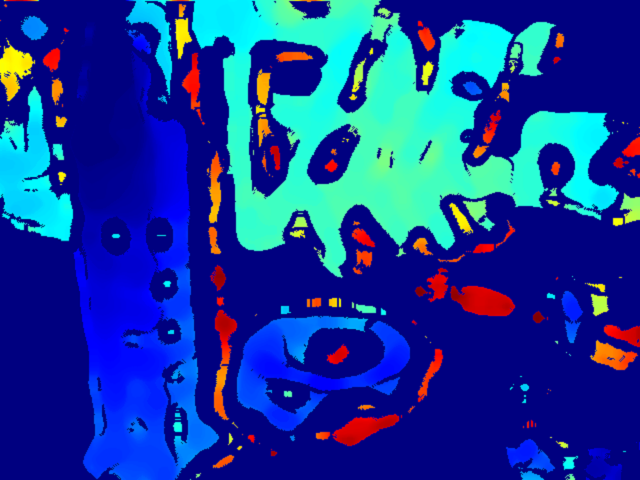
\includegraphics[width=6cm]{images/methodology/FVR/home_depth_frame_mono}
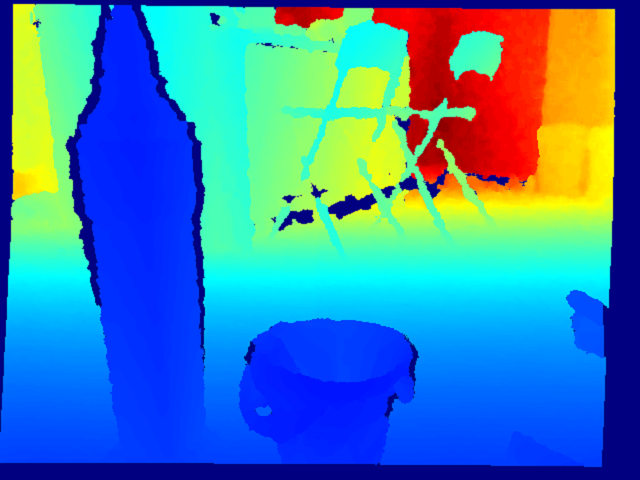
\includegraphics[width=6cm]{images/methodology/FVR/home_depth_frame}
\caption{Comparison between block matching estimated depth (left) and RGBD device depth (right).}
\label{fig:DepthGenerationExample}
\end{figure}
 
\subsubsection{Limitations of MVVR}

During experiments it was discovered that due to the high levels of noise, the MVVR method was limited to registration of translation information only. This was due to the difficulty in computing depth data using basic methods such as stereo methods between frames and optical flow. Despite this limitation, the FVR method was able to register up to 15 centimetres of camera translation (see experiments in section \ref{Sec:MonocularExperimentsSection}).  